\documentclass[conference]{IEEEtran}

\usepackage{hyperref}
\usepackage{graphicx}
\usepackage{amsmath}
%\usepackage[backend=biber, style=alphabetic]{biblatex}

%\usepackage{authblk}

%\addbibresource{./citations.bib}

\title{CHILLAX - at Arabic Hate Speech 2022: Detect Hate Speech using Logistic Regression and Random Forest}

\author{Prof Ensaf Hussein \\Kirollos Hany, Kirollos George, Malak Emad, \\ Shady Zekry, Seif Hesham, Fady Fayek}
\date{}

\graphicspath{{graphics/}}

\begin{document}
	
\nocite{*}
	
\maketitle

\begin{abstract}
	Hate speech and offensive language became a crucial problem nowadays due to the large usage of social media by people from different gender, nationality, religion and other types of characteristics allowing anyone to share their thoughts and opinions. In this research paper we experiment the result of using the Arabic pretrained Bert language model MARBERT for feature extraction of the Arabic tweets in the dataset provided by OSACT2022 shared task then feeding the features to classic machine learning models (Logistic Regression, Random Forest). The best results achieved were by the Logistic Regression model with accuracy, precision, recall, and f1-score of 0.8, 0.78, 0.78, and 0.78 for the offensive tweet detection task respectively and for the hate speech tweet detection task results achieved were 0.89, 0.72, 0.8, and 0.76 these results were achieved on the OSACT2022 test dataset.
\end{abstract}

\section{Introduction}

Pre-trained language models based on Transformer~\cite{vaswani2017attention} such as GPT~\cite{radford2018improving}, Bert~\cite{devlin2018bert}, XLNet ~\cite{yang2019deepening}, and RoBERTa~\cite{zhuang2021robustly} have been shown to be effective for learning contextualized language representation achieving state-of-the-art results on a wide variety of natural language processing tasks.
Recent research have adopted the methodology of fine tuning a pretrained language model by simply adding a fully connected neural layer specific to the down-stream task the model is being fine tuned for such as sarcasm detection~\cite{farha2021benchmarking} and hate speech detection~\cite{aldjanabi2021arabic}. Research have shown that due to the numerous layers present in Transformer models simply feeding the output of the Transformer’s encoder final layer to the fully connected neural layer would restrict the power of the pretrained representations of the language~\cite{yang2019deepening}.~\cite{devlin2018bert} shows that different combinations of different output layers of the Transformers encoder layers result in distinct performance on different tasks like Named Entity Recognition task. It is found that the most contextualized representations of input text tend to occur in the middle layers, while top layers are for language modeling~\cite{yang2019deepening}. We explore the results of obtaining the text representation from different combination of layers of the Transformers encoder layers then using it as features for classical machine learning models (Logistic Regression, Random Forest) for both of the OSACT2022 shared tasks which is Arabic offensive and hate speech tweets detection. We used the MARBERT pretrained Transformer model as it were trained on a large Arabic tweets corpora and have proved to be efficient in similar tasks such as sentiment analysis where it scored 0.93 F1-score on ArSAS dataset~\cite{abdul-mageed-etal-2021-arbert}. We experimented on the OSACT2022 shared task dataset, which had a class imbalance problem present in both tasks offensive and hate speech detection we tackled the problem by using data augmentation techniques to achieve a balanced class distribution in the dataset to prevent the classifiers from biasing towards the majority class. The research paper is organized as follows. Section II gives a brief overview of related work. Section III explains in details our methodology and proposed model. Section IV presents the experiment results  and evaluation metrics. Section V concludes our research and our potential future work.


\section{Related Work}
%Our goal in this task was to find the best approach to tackle the problem. First trying we have used tfidf technique, but the problem was that model was detecting words by its own meaning only without looking how it would be helpful for the context. Second method we moved into using MARbert after searching for a method that helps in understanding the whole paragraphs and give the meaning for each word. It is made by extracting every single word as a vector in vector space representing in our case tweets. Then the method we used MARbert is by extracting features for our Logistic Regression model or our Random Forest model. The most appealing results relatively appeared in Random Forest model with results: 79\%, 85\% and 82\% for precision, recall and f1-score for not offensive tweets and 83\%, 76\% and 79\% for precision, recall and f1-score for Logistic Regression, and for Random Forest 90\%, 91\% and 91\% for precision, recall and f1-score for not hate speech tweets and 91\%, 90\% and 91\% for precision, recall and f1-score. One of the challenges we have faced that data we used in training was heavily biased towards not-offensive hate speech tweets, so after a lot of researching we have used NLP Augmenter to generate new hate speech tweet to balance the data.

Recently, the interest in detecting hate speech has increased rapidly attracting the attention of many researchers trying to develop various models and methods to extract hate features and hateful content. There are several research studies conducted to study hate speech and offensive language in online communities and social media over Arabic content.~\cite{abuzayed2020quick} investigate 15 classical and neural learning models with TF-IDF and word embedding as feature representations of the OSACT-2020 dataset their best classifier (A joint architecture of CNN and RNN) achieved 0.73 macro F1-score on the development dataset and 0.69 on the test dataset with word embedding as feature representations.~\cite{alshaalan2020hate} investigate several neural network models that are based on CNN and RNN to detect hate speech in Arabic tweets and also evaluates recent BERT model on the task of Arabic hate speech detection. They build a hate speech dataset containing 9,316 annotated Arabic tweets and conducted experiments on that dataset and an out-domain dataset showing that the CNN model achieves an F1-score of 0.79 and AUROC of 0.89.~\cite{faris2020hate} proposed a smart deep learning approach for the detection of cyber hate speech. The detection of hate speech on Twitter on the Arabic region in particular using a word embedding mechanism for feature representation and fed to a hybrid CNN and LSTM neural network that achieved a 0.71 F1-score on a dataset that is collected from the Twitter API.~\cite{al2020hate} collected a 3,000 tweet dataset from Twitter where they experimented BOW and TF-IDF methods for feature representation and classical machine learning models (SVM, NB, RF) and concluded that TF-IDF with SVM achieved the best results of 0.82 F1-score.


\section{Methods and Materials}
\subsection{The dataset}
We used the Arabic tweets dataset provided by OSACT2022 shared task which contains around 13,000 tweets in total where 35\% are offensive and 11\% are hate speech. Vulgar and violent tweets represents 1.5\% and 0.7\% of the dataset respectively. The dataset were split into 3 parts train, development, and test with percentages 70\%, 10\%, and 20\% respectively. For our first task which is offensive tweet detection the train dataset contained 5,715 offensive and 3,172 not offensive tweets figure 1 contains the count plot showing the class imbalance presented in the train dataset for our first task. For our second task which is hate speech tweet detection the train dataset contained 7,928 not hate speech and 959 hate speech tweets which shows a big class imbalance for this task figure 2 contains the count plot showing the class imbalance presented in train dataset for our second task.

%Then after applying the NLP aug ~\cite{al2020hate}, the data set was balanced in a reasonable manner.

\begin{figure}[htbp]
	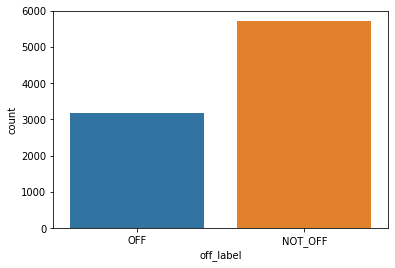
\includegraphics[width=\columnwidth, height=0.22\paperheight]{01.png}
	\caption{Offensive detection task label count plot}
	\label{fig:off_plot}
\end{figure}

\begin{figure}[htbp]
	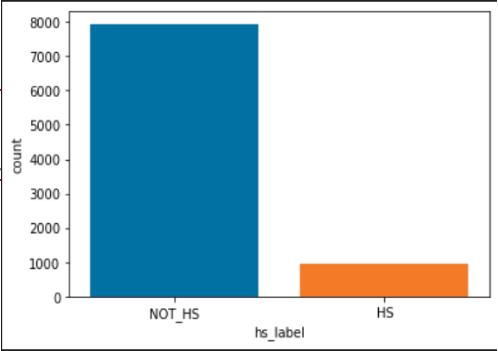
\includegraphics[width=\columnwidth, height=0.30\paperwidth]{07.png}
	\caption{Hate speech detection task label count plot}
	\label{fig:hate_speech}
\end{figure}

The data set we have used we split it into 2 parts. First part is testing data which is 70\%, and testing data which represents 30\%. Worth mentioning that the data set is from the \href{https://sites.google.com/view/arabichate2022/home}{competition}.

\section{Proposed Model}

\begin{figure}[htbp]
	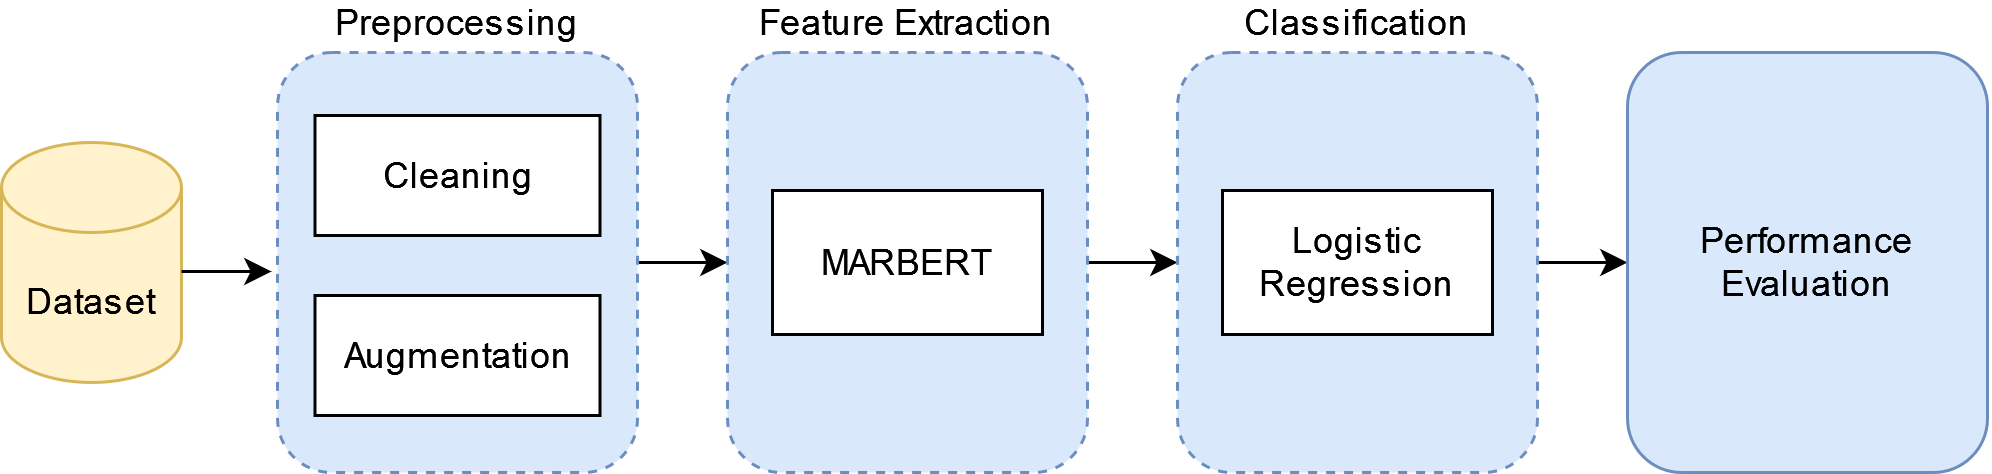
\includegraphics[width=\columnwidth, height=0.04\textheight]{04.png}
%	\caption{text}
\end{figure}

\subsection{Preprocessing}
For the preprocessing phase all URLs and user mentions were removed from the tweet text. To tackle the class imbalance problem present in the two tasks contextual word embedding with insert action data augmentation technique using MARBERT Arabic model to generate new tweets of the minority classes (offensive, hate speech) so that the class distribution in both tasks were balanced to prevent the model from biasing towards the majority classes (not offensive, not hate speech). Some of the augmented tweets had an unknown special token generated these tokens were removed from the augmented tweets. The NLP aug ~\cite{al2020hate} data augmentation library were used for the data augmentation. Figure~\ref{fig:aug_off_tweets} and~\ref{fig:aug_hate_tweets} shows a sample of augmented offensive and hate speech tweets respectively.

\begin{figure}[htbp]
	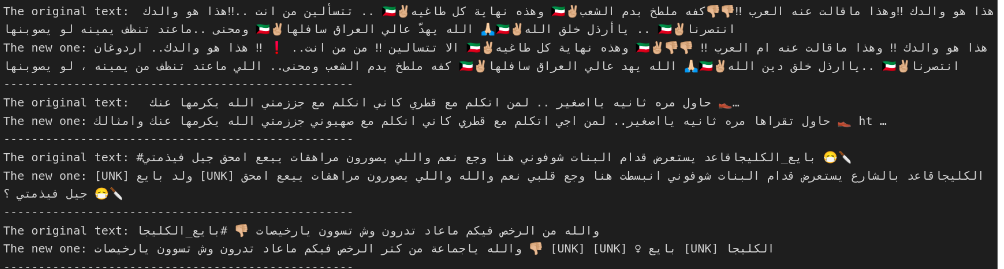
\includegraphics[width=\columnwidth, height=0.11\paperheight]{05.png}
	\caption{Augmented offensive tweets sample}
	\label{fig:aug_off_tweets}
\end{figure}

\begin{figure}[htbp]
	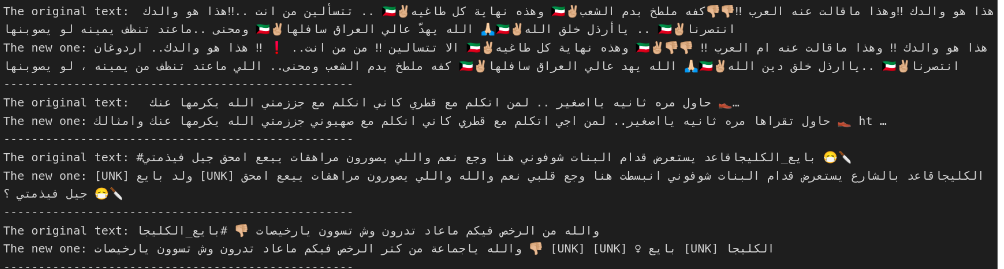
\includegraphics[width=\columnwidth, height=0.11\paperheight]{05.png}
	\caption{Augmented hate speech tweets sample}
	\label{fig:aug_hate_tweets}
\end{figure}

\subsection{Feature Extraction}
For the feature extraction phase we used MARBERT pretrained Arabic language model to extract features which will be later fed to the machine learning models Logistic Regression and Random Forest for training. The MARBERT model is a Bert-base model which consists of 12 hidden layers and hidden size of 768 the output of the last four hidden layers where each layer is of dimensions sentence length x hidden size were obtained then the the output of each layer is summed to produce a single vector of sentence length x hidden size dimensions then the mean of this vector was computed to produce a single vector of hidden size length which represents the feature vector for the tweet that will be fed to the machine learning models.

\subsection{Training}
Scikit-Learn library implementation of Logistic Regression and Random Forest were used in training phase. For the Logistic Regression model a C parameter of 1e-3 and saga solver were used. For the Random Forest Model a max sample parameter of 0.4 was used.

\section{Results and Performance Evaluation}
Before training the model the train dataset were split into 70\% for training and 30\% for testing to use for evaluating the model along with the development and test datasets that were provided by the OSACT2022 shared task.


\subsection{Performance Evaluation Metrics}
The evaluation metrics used are macro averaged Precision, Recall, F1-score, and Accuracy where Precision is the fraction of classified tweets that are relevant which is formulated in equation~\ref{eq:precision}. Recall is the fraction of relevant tweets that are classified which is formulated in equation~\ref{eq:recall}. F1-score is the mean of precision and recall which is formulated in equation~\ref{eq:f1_score}. Accuracy the fraction of correct tweets that have been classified from actual classes as shown in Equation~\ref{eq:accuracy}.

\begin{align}\label{eq:precision}
	\text{Precision} = \dfrac{TP}{TP + FP}
\end{align}
\begin{align}\label{eq:recall}
	\text{Recall}=\dfrac{TP}{TP + FN}
\end{align}
\begin{align}\label{eq:f1_score}
	\text{f1-score}=\dfrac{2 \times \text{Precision} \times \text{Recall }}{\text{Precision} + \text{Recall} }
\end{align}
\begin{align}\label{eq:accuracy}
	\text{Accuracy} = \dfrac{TP + TN}{TP + FP + TN + FN}
\end{align}

where:


True Positive (TP): refers to a set of tweets that have been classified correctly to the task class (offensive, hate speech).


False Positive (FP): refers to a set of tweets that have been classified incorrectly and have been said to be related to the task class (offensive, hate speech) incorrectly.


True Negative (TN): refers to a set of tweets that have not been classified into the task class (offensive, hate speech) and are actually not labeled as task class (offensive, hate speech).


False Negative (FN): refers to a set of tweets that have not been classified correctly and have been said to be non-related to the task class (offensive, hate speech) but they are actually labeled as task class (offensive, hate speech).

\subsection{Results}

The baselines for evaluation provided by OSACT2022 are as following:

\begin{table}[htbp]
	\begin{tabular}{|c|c|c|c|c|}
		\hline
		Task & Accuracy & Precision & Recall & f1-score \\ \hline
		Offensive detection & 0.65 & 0.65 & 0.65 & 0.65 \\ \hline
		Hate speech detection & 0.89 & 0.89 & 0.89 & 0.89 \\ \hline
	\end{tabular}
\end{table}

The results obtained for each model and dataset for the offensive detection task are as following:

\begin{table}[htbp]
	\begin{tabular}{|c|c|c|c|c|c|}
		\hline
		Model & Dataset & Accuracy & Precision & Recall & f1-score \\ \hline
		Logistic Regression & Train & 0.85 & 0.85 & 0.85 & 0.85 \\ \hline
		Logistic Regression & Test(30\% of train) & 0.81 & 0.81 & 0.81 & 0.81 \\ \hline
		Logistic Regression & Development & 0.8 & 0.77 & 0.78 & 0.78 \\ \hline
		Logistic Regression & OSACT2022-Test & 0.8 & 0.78 & 0.78 & 0.78 \\ \hline
		Random Forest & Train & 0.97 & 0.97 & 0.97 & 0.97 \\ \hline
		Random Forest & Test(30\% of train) & 0.77 & 0.77 & 0.77 & 0.77 \\ \hline
		Random Forest & Development & 0.75 & 0.72 & 0.73 & 0.72 \\ \hline
		Random Forest & OSACT2022-Test & 0.74 & 0.72 & 0.72 & 0.72 \\ \hline
	\end{tabular}
\end{table}

The results obtained for each model and dataset for the hate speech detection task are as following:

\begin{table}[htbp]
	\begin{tabular}{|c|c|c|c|c|c|}
		\hline
		Model & Dataset & Accuracy & Precision & Recall & f1-score \\ \hline
		Logistic Regression & Train & 0.91 & 0.91 & 0.91 & 0.91 \\ \hline
		Logistic Regression & Test(30\% of train) & 0.91 & 0.91 & 0.91 & 0.91 \\ \hline
		Logistic Regression & Development & 0.89 & 0.7 & 0.81 & 0.74 \\ \hline
		Logistic Regression & OSACT2022-Test & 0.89 & 0.73 & 0.81 & 0.76 \\ \hline
		Random Forest & Train & 0.98 & 0.98 & 0.98 & 0.98 \\ \hline
		Random Forest & Test(30\% of train) & 0.9 & 0.9 & 0.9 & 0.9 \\ \hline
		Random Forest & Development & 0.87 & 0.67 & 0.81 & 0.7 \\ \hline
		Random Forest & OSACT2022-Test & 0.87 & 0.69 & 0.79 & 0.73 \\ \hline
	\end{tabular}
\end{table}

\section{Conclusion}
We present an approach to detect Hate speech texting detection based on natural language processing.our approach can be applied to detecting hate speech dialogue which is composed of pure text.
The challenge was to find a way to detect hate speech in the Arabic language, as the data set imbalanced, and we overcame that by using the data augmentation method and NLP aug ~\cite{al2020hate} tool helped us.
Using logistic regression and marbert as feature extraction we got 91\%, 90\% and 91\% for precision, recall and f1-score for hate speech tweets.
Furthermore, we aim to develop a more balanced dataset and execute the algorithm in a real environment. The results will indicate if any new algorithms might be necessary to improve
detection.


%
% Starting bibliography
%

\clearpage
\onecolumn

\bibliographystyle{plain}
\bibliography{./citations.bib}

\end{document}
